%=========================================================
\chapter{Modelo dinámico}	
\label{cap:modDinamico}

	Este capítulo describe en modelo dinámico del sistema. en el se detallan todos los escenarios de ejecución del sistema. La figura~\ref{fig:casosDeUso} muestra el diagrama general del sistema y sus sib sistemas, y la figura~\ref{fig:casosDeUsoDetalle} muestra todos los casos de uso del sistema. En este documento solo detallamos los casos de uso del subsistema de gestión de cursos.
	
\begin{figure}[htbp]
	\begin{center}
		\fbox{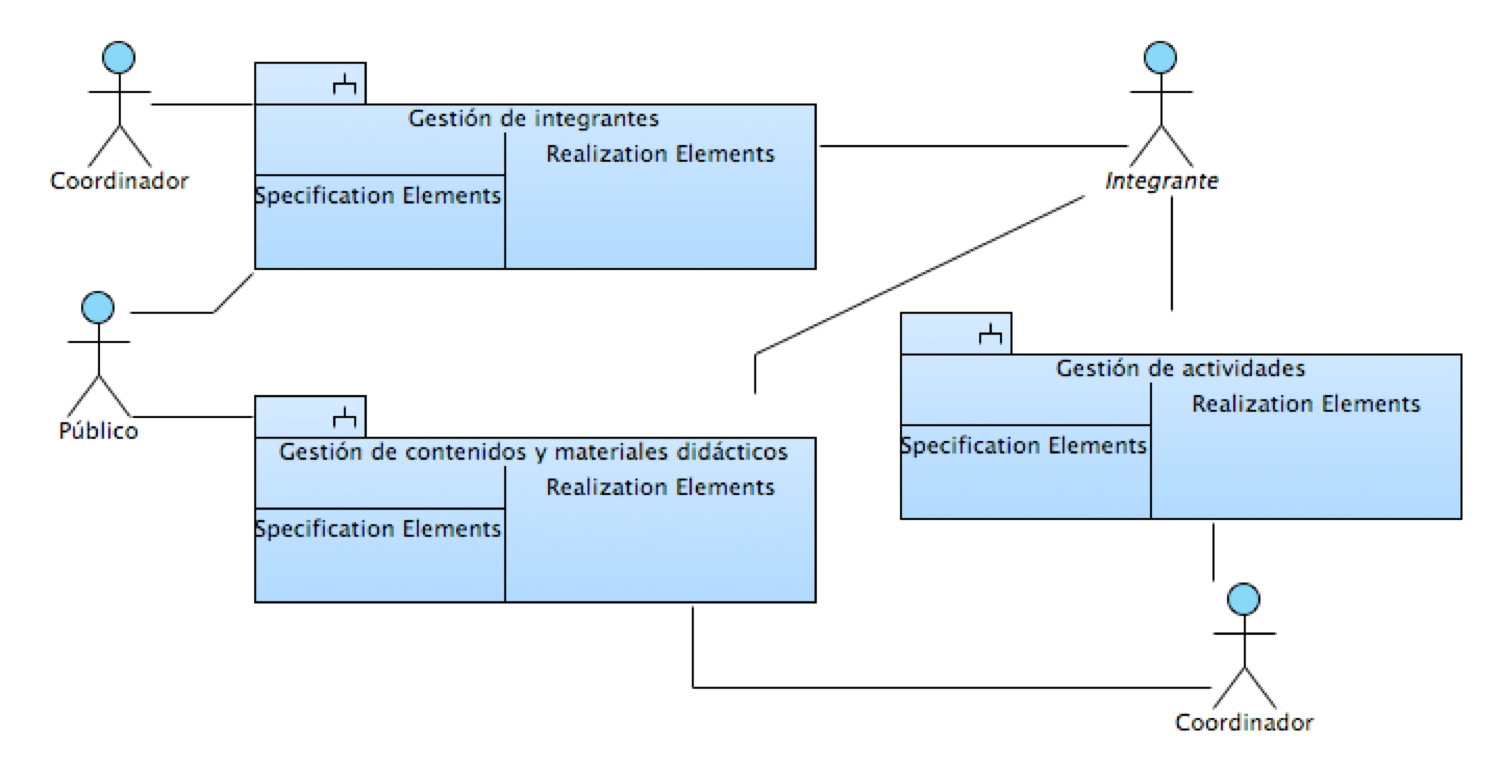
\includegraphics[width=.8\textwidth]{images/casosDeUso}}
		\caption{Diagrama de casos de uso del sistema.}
		\label{fig:casosDeUso}
	\end{center}
\end{figure}

\begin{figure}[htbp]
	\begin{center}
		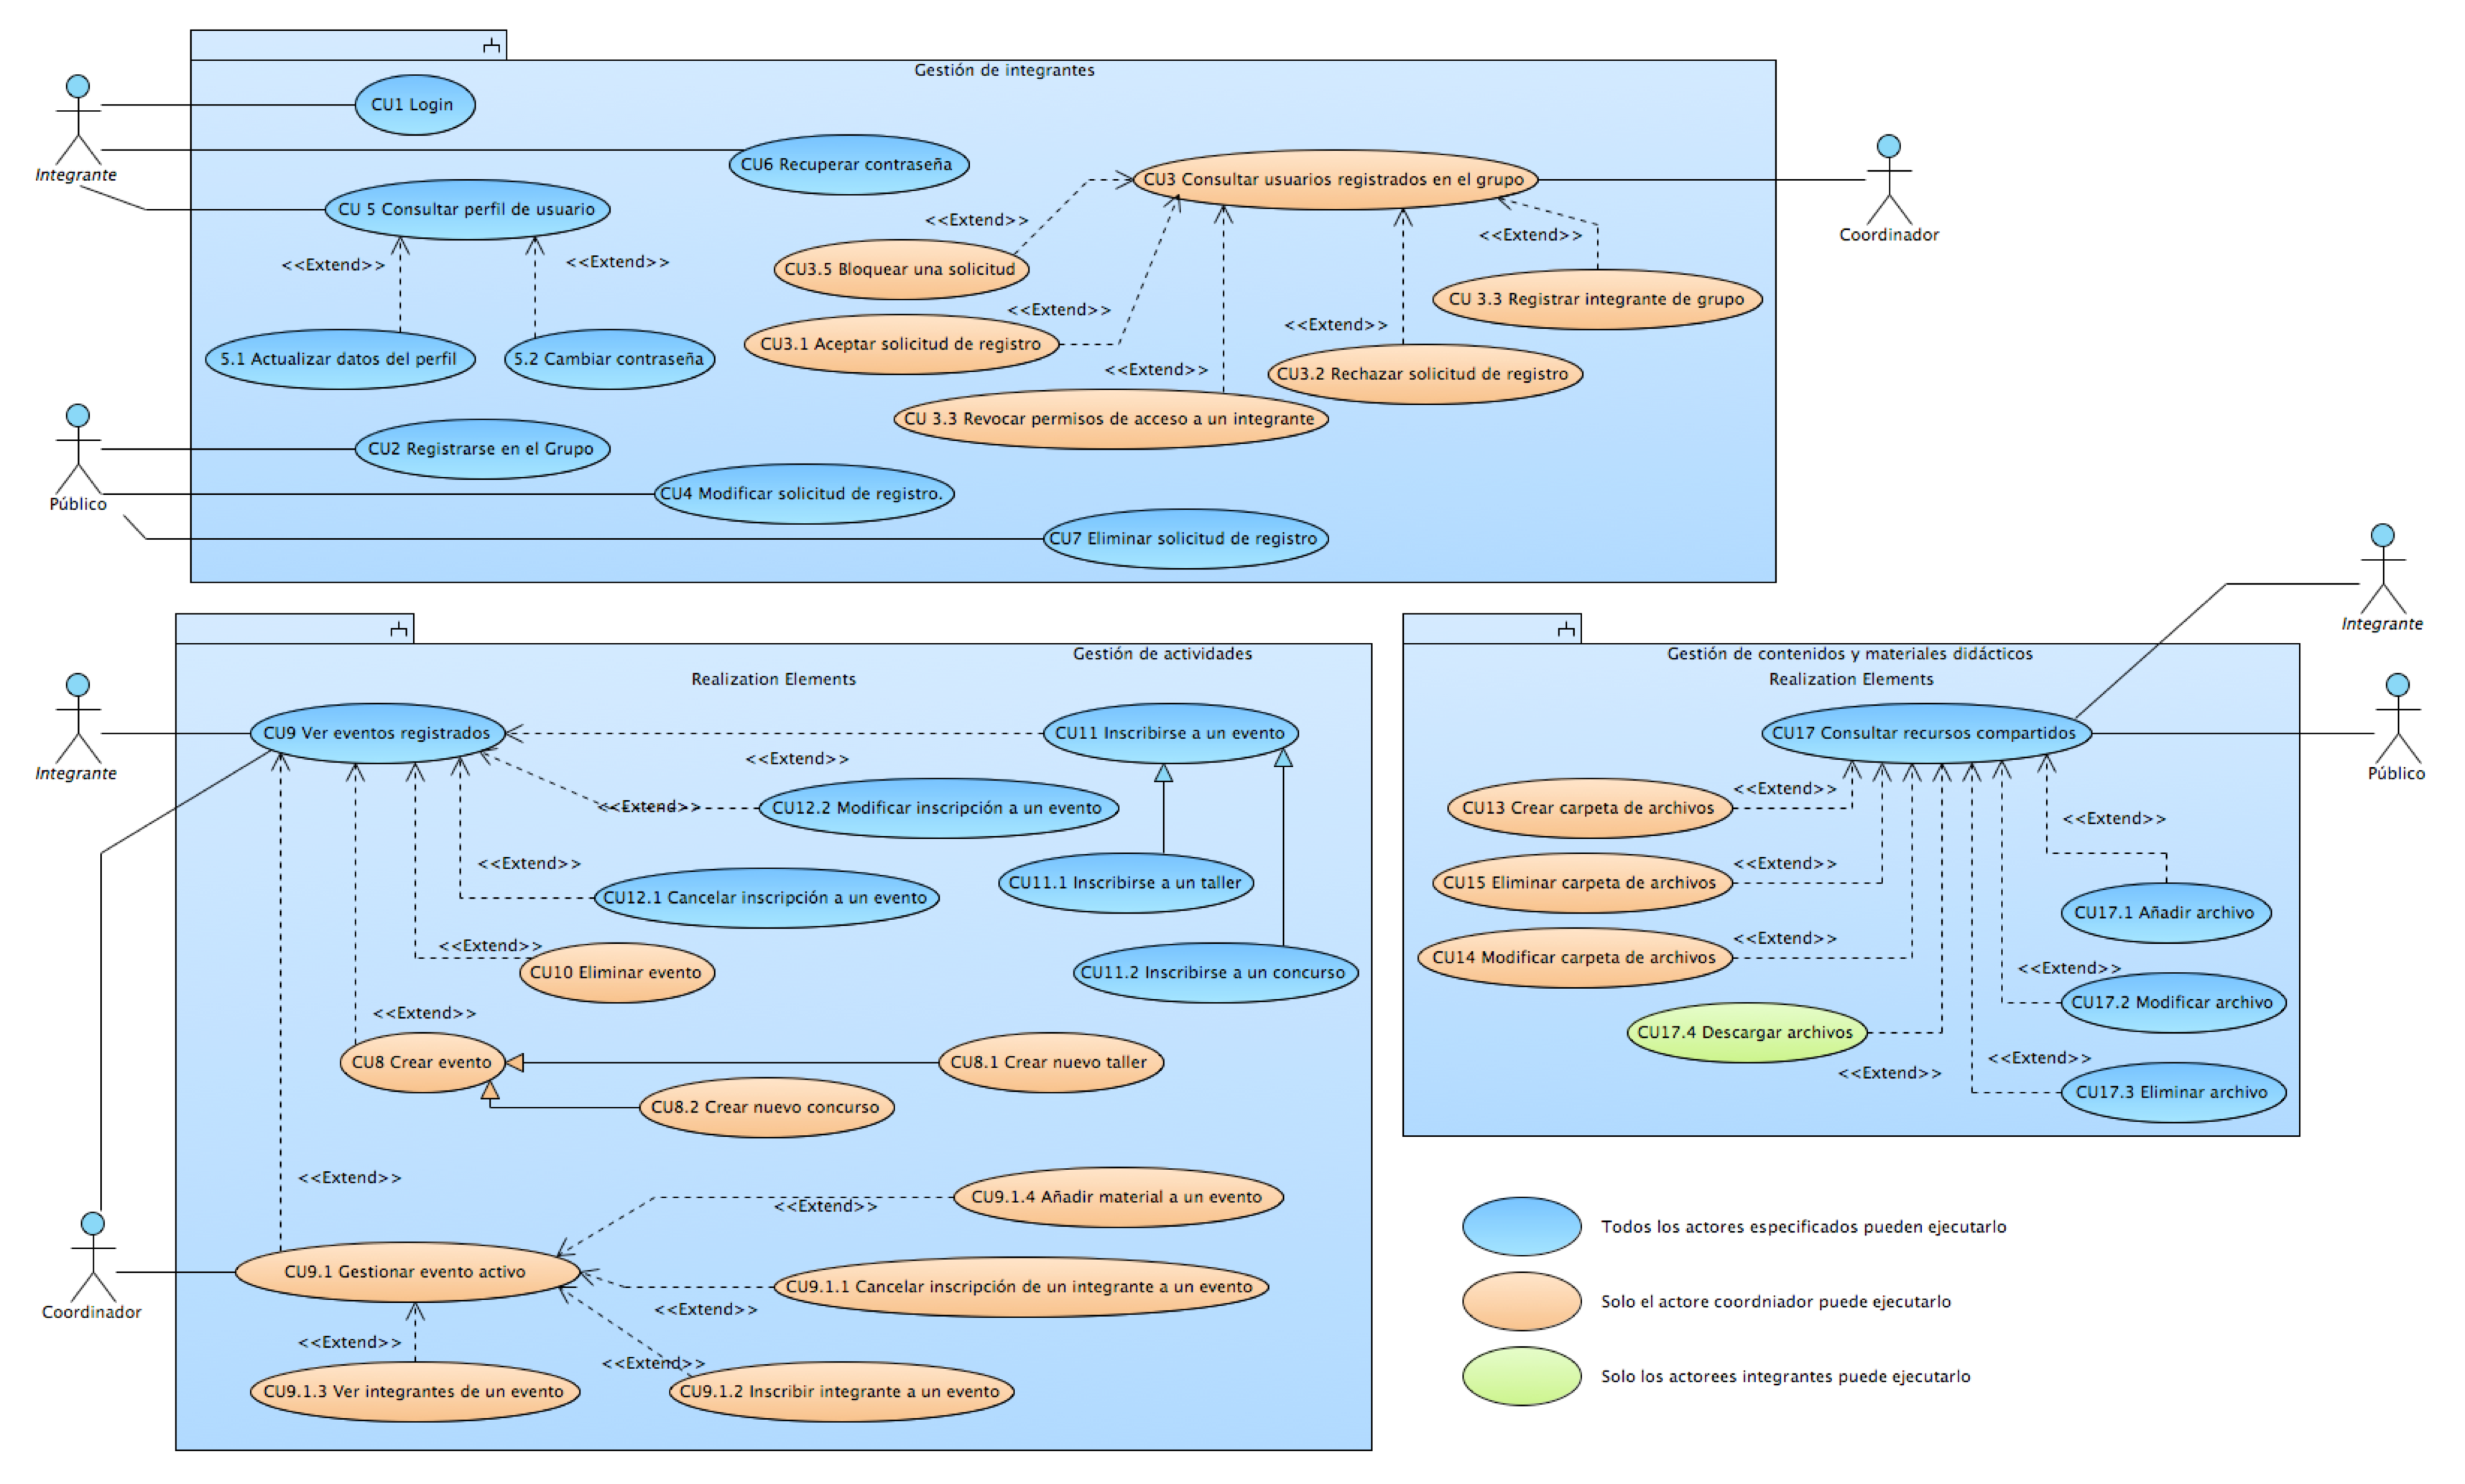
\includegraphics[angle=90, width=.7\textwidth]{images/casosDeUsoDetalle}
		\caption{Diagrama detallado del sistema.}
		\label{fig:casosDeUsoDetalle}
	\end{center}
\end{figure}

%---------------------------------------------------------
\section{Descripción de actores}

%---------------------------------------------------------
\begin{Usuario}{\hypertarget{getenteOperaciones}{\subsection{Gerente de Operaciones}}}{
	Es el encargado de todas las operaciones de la empresa y está por encima de los ejecutivos de producción y de ventas principalmente.
}
    \item[Responsabilidades:] \cdtEmpty
    \begin{itemize}
		\item Supervisar la operación.
		\item Plantear y supervisar el logro de las metas de la empresa y su crecimiento económico.
		\item ...
    \end{itemize}

	\item[Perfil:] \cdtEmpty
    \begin{itemize}
		\item Amplia experiencia en el ramo.
		\item Licenciatura como mínimo.
		\item ...
    \end{itemize}
\end{Usuario}

A continuación se detallan los casos de uso.

%---------------------------------------------------------
% CASOS DE USO

% \IUref{IUAdmPS}{Administrar Planta de Selección}
% \IUref{IUModPS}{Modificar Planta de Selección}
% \IUref{IUEliPS}{Eliminar Planta de Selección}

% 


% Copie este bloque por cada caso de uso:
%-------------------------------------- COMIENZA descripción del caso de uso.

%\begin{UseCase}[archivo de imágen]{UCX}{Nombre del Caso de uso}{
%--------------------------------------
	\begin{UseCase}{CU1}{Iniciar Sesión}{
		Este caso de usos permite al usuario iniciar sesión en el sistema para poder visualizar los Exámenes a Título de Suficiencia (ETS).
	}
		\UCitem{Actor}{\hyperlink{Alumno}{Alumno, Personal de seguridad, Docente}}
		\UCitem{Propósito}{Permitir al usuario ingresar al sistema.}
		\UCitem{Entradas}{Número de boleta (en caso de ser alumno), RFC (en caso de ser del Personal de seguridad o Docente) y Contraseña.}
		\UCitem{Origen}{Teclado}
		\UCitem{Salidas}{-}
		\UCitem{Destino}{Pantalla principal del sistema}
		\UCitem{Precondiciones}{El usuario deberá estar registrado en el sistema SAES.}
		\UCitem{Postcondiciones}{El usuario podrá acceder a la funcionalidad del sistema.}
		\UCitem{Errores}{Es posible que al intentar iniciar sesión se presenten los siguientes inconvenientes: 
			\begin{itemize}
				\item El usuario ingresa sus credenciales incorrecta. 
				\item El usuario no llena todos lo campos obligatorios. 
			\end{itemize}
		}
		\UCitem{Tipo}{Caso de uso primario}
		\UCitem{Observaciones}{}
	\end{UseCase}
%--------------------------------------
	\begin{UCtrayectoria}
		\UCpaso[\UCactor] Introduce su Número de Boleta en caso de ser alumno o su RFC en caso de ser Docente o Personal de seguridad y Contraseña en el sistema vía la  \IUref{IU1}{Pantalla de Inicio de sesión}\label{CU01Login}.
		\UCpaso[\UCactor] Confirma la operación presionando el botón \IUbutton{Iniciar Sesión}.
		\UCpaso Verifica que los datos ingresados coincidan con algún registro guardado dentro del sistema SAES con base en la regla \BRref{BR129}{Determinar.} \Trayref{A} \Trayref{B}.
		\UCpaso Despliega la \IUref{IU02}{Pantalla principal} con la lista de opciones disponible que tiene cada usuario.
	\end{UCtrayectoria}

%--------------------------------------		
		\begin{UCtrayectoriaA}{A}{El Estudiante intenta iniciar sesión , pero el Número de boleta o RFC o contraseña no coincide con algún registro dentro de la base de datos}
			\UCpaso Muestra el Mensaje {\bf MSG1-}``El usuario [{\em Número de Boleta o RFC}] no coincide con ninguna cuenta. Verifique la información e intente de nuevo''.
			\UCpaso[\UCactor] Oprime el botón \IUbutton{Aceptar}.
			\UCpaso[] Termina el caso de uso.
		\end{UCtrayectoriaA}
		

%--------------------------------------
% Puntos de extensión
\subsection{Puntos de extensión}
\UCExtenssionPoint{
	% Cuando:
	Desea conocer las materias cursadas.
}{
	% Durante la región:
	Del paso 4 al paso 9.
}{
	% Casos de uso a los que extiende:
	\hyperlink{CU3.4}{CU3.4 Consultar historial académico}.
}
		
		
		
%-------------------------------------- TERMINA descripción del caso de uso.



